\documentclass[crop,tikz]{standalone}% 'crop' is the default for v1.0, before it was 'preview'
%\usetikzlibrary{...}% tikz package already loaded by 'tikz' option

\usetikzlibrary{arrows,positioning} 
\usetikzlibrary{shapes,decorations}
\usetikzlibrary{calc}
\usetikzlibrary{fit}
\usetikzlibrary{decorations.pathreplacing}
\usetikzlibrary{backgrounds}


\renewcommand{\familydefault}{\sfdefault}


\definecolor{blind_red}{HTML}{D7191C}
\definecolor{blind_orange}{HTML}{FDAE61}
\definecolor{blind_yellow}{HTML}{FFFFBF}
\definecolor{blind_blue}{HTML}{ABD9E9}
\definecolor{blind_blue2}{HTML}{2C7BB6}



\begin{document}
	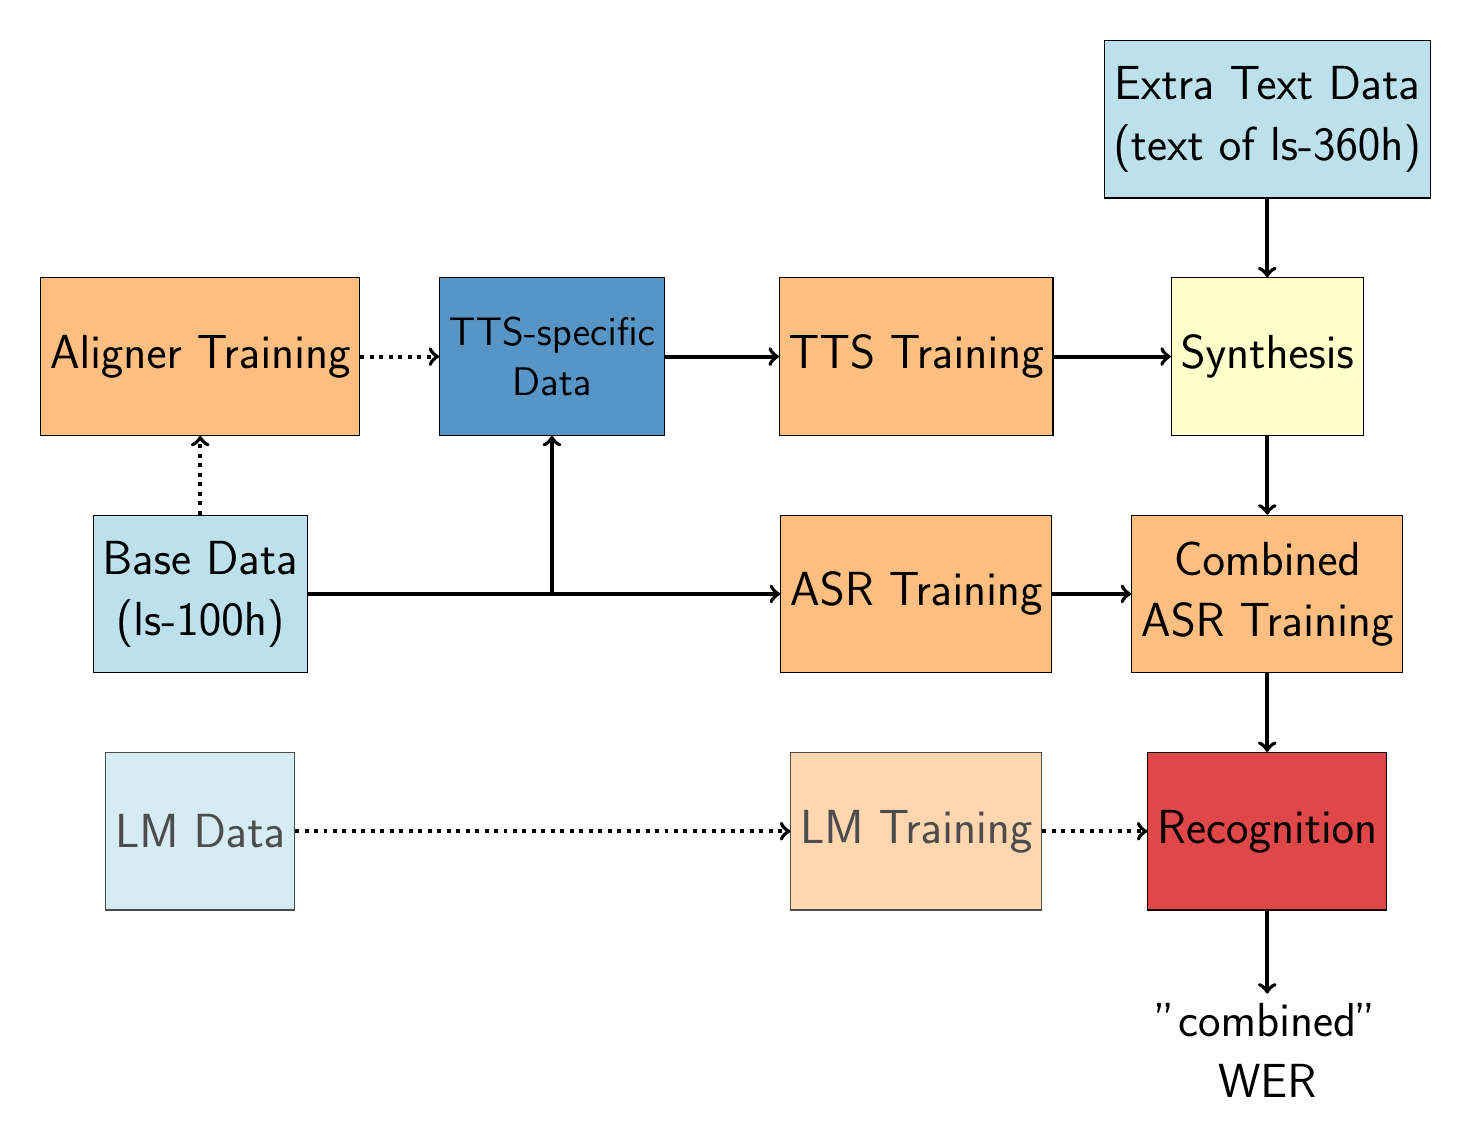
\begin{tikzpicture}[
	    auto,
	    background rectangle/.style={fill=white}, show background rectangle,
	    onlytext/.style={align=center, font=\LARGE},
        halfbox/.style={rectangle, minimum size=1.20cm, draw, font=\LARGE},
	    box/.style={rectangle, minimum size=2.00cm, draw, font=\LARGE},
	    halforangebox/.style={halfbox, fill=blind_orange!80},
	    orangebox/.style={box, fill=blind_orange!80},
	    normalline/.style={->, line width=0.5mm},
	    state/.style={rectangle, draw, minimum height=0.8cm, minimum width=0.2cm},
	]
		\node[box, fill=blind_blue!80, align=center] (basedata) at (0, 0) {Base Data\\(ls-100h)};
        \node[orangebox, above=1cm of basedata, align=center] (aligner) {Aligner Training};
        \node[box, fill=blind_blue2!80, right=1cm of aligner, align=center, font=\Large] (ttsdata) {TTS-specific \\ Data};
        \node[orangebox, right=6cm of basedata, align=center] (asr) {ASR Training};
        \node[orangebox, above=1cm of asr, align=center] (tts) {TTS Training};
        \node[orangebox, right=1cm of asr, align=center] (contasr) {Combined \\ ASR Training};
        \node[box, fill=blind_yellow!80, above=1cm of contasr, align=center] (synth) {Synthesis};
        \node[box, fill=blind_blue!80, above=1cm of synth, align=center] (extradata) {Extra Text Data\\(text of ls-360h)};

        \node[box, color=black!70, fill=blind_blue!50, below=1cm of basedata, align=center] (lmdata) {LM Data};
        \node[box, color=black!70, fill=blind_orange!50, below=1cm of asr, align=center] (lm) {LM Training};
        \node[box, fill=blind_red!80, below=1cm of contasr, align=center] (recog) {Recognition};

         \node[onlytext, below=30pt of recog] (wer) {"combined"\\ WER};

        \draw [normalline, dotted] (basedata) -- (aligner);
        \draw [normalline, dotted] (aligner) -- (ttsdata);
        \draw [normalline] (ttsdata) -- (tts);
        \draw [normalline] (tts) -- (synth);
        \draw [normalline] (extradata) -- (synth);

        \draw [normalline] (basedata) -- (asr);
		\draw let \p1 = (basedata), \p2 = (ttsdata) in [normalline] (\x2, \y1) -- (ttsdata.south);

        \draw [normalline] (asr) -- (contasr);
		\draw [normalline] (synth) -- (contasr);
        \draw [normalline, dotted] (lmdata) -- (lm);
		\draw [normalline] (contasr) -- (recog);
		\draw [normalline, dotted] (lm) -- (recog);
		\draw [normalline] (recog) -- (wer);
	\end{tikzpicture}
\end{document}